\documentclass[twoside]{book}

% Packages required by doxygen
\usepackage{fixltx2e}
\usepackage{calc}
\usepackage{doxygen}
\usepackage[export]{adjustbox} % also loads graphicx
\usepackage{graphicx}
\usepackage[utf8]{inputenc}
\usepackage{makeidx}
\usepackage{multicol}
\usepackage{multirow}
\PassOptionsToPackage{warn}{textcomp}
\usepackage{textcomp}
\usepackage[nointegrals]{wasysym}
\usepackage[table]{xcolor}

% Font selection
\usepackage[T1]{fontenc}
\usepackage[scaled=.90]{helvet}
\usepackage{courier}
\usepackage{amssymb}
\usepackage{sectsty}
\renewcommand{\familydefault}{\sfdefault}
\allsectionsfont{%
  \fontseries{bc}\selectfont%
  \color{darkgray}%
}
\renewcommand{\DoxyLabelFont}{%
  \fontseries{bc}\selectfont%
  \color{darkgray}%
}
\newcommand{\+}{\discretionary{\mbox{\scriptsize$\hookleftarrow$}}{}{}}

% Page & text layout
\usepackage{geometry}
\geometry{%
  a4paper,%
  top=2.5cm,%
  bottom=2.5cm,%
  left=2.5cm,%
  right=2.5cm%
}
\tolerance=750
\hfuzz=15pt
\hbadness=750
\setlength{\emergencystretch}{15pt}
\setlength{\parindent}{0cm}
\setlength{\parskip}{3ex plus 2ex minus 2ex}
\makeatletter
\renewcommand{\paragraph}{%
  \@startsection{paragraph}{4}{0ex}{-1.0ex}{1.0ex}{%
    \normalfont\normalsize\bfseries\SS@parafont%
  }%
}
\renewcommand{\subparagraph}{%
  \@startsection{subparagraph}{5}{0ex}{-1.0ex}{1.0ex}{%
    \normalfont\normalsize\bfseries\SS@subparafont%
  }%
}
\makeatother

% Headers & footers
\usepackage{fancyhdr}
\pagestyle{fancyplain}
\fancyhead[LE]{\fancyplain{}{\bfseries\thepage}}
\fancyhead[CE]{\fancyplain{}{}}
\fancyhead[RE]{\fancyplain{}{\bfseries\leftmark}}
\fancyhead[LO]{\fancyplain{}{\bfseries\rightmark}}
\fancyhead[CO]{\fancyplain{}{}}
\fancyhead[RO]{\fancyplain{}{\bfseries\thepage}}
\fancyfoot[LE]{\fancyplain{}{}}
\fancyfoot[CE]{\fancyplain{}{}}
\fancyfoot[RE]{\fancyplain{}{\bfseries\scriptsize Generated by Doxygen }}
\fancyfoot[LO]{\fancyplain{}{\bfseries\scriptsize Generated by Doxygen }}
\fancyfoot[CO]{\fancyplain{}{}}
\fancyfoot[RO]{\fancyplain{}{}}
\renewcommand{\footrulewidth}{0.4pt}
\renewcommand{\chaptermark}[1]{%
  \markboth{#1}{}%
}
\renewcommand{\sectionmark}[1]{%
  \markright{\thesection\ #1}%
}

% Indices & bibliography
\usepackage{natbib}
\usepackage[titles]{tocloft}
\setcounter{tocdepth}{3}
\setcounter{secnumdepth}{5}
\makeindex

% Hyperlinks (required, but should be loaded last)
\usepackage{ifpdf}
\ifpdf
  \usepackage[pdftex,pagebackref=true]{hyperref}
\else
  \usepackage[ps2pdf,pagebackref=true]{hyperref}
\fi
\hypersetup{%
  colorlinks=true,%
  linkcolor=blue,%
  citecolor=blue,%
  unicode%
}

% Custom commands
\newcommand{\clearemptydoublepage}{%
  \newpage{\pagestyle{empty}\cleardoublepage}%
}

\usepackage{caption}
\captionsetup{labelsep=space,justification=centering,font={bf},singlelinecheck=off,skip=4pt,position=top}

%===== C O N T E N T S =====

\begin{document}

% Titlepage & ToC
\hypersetup{pageanchor=false,
             bookmarksnumbered=true,
             pdfencoding=unicode
            }
\pagenumbering{roman}
\begin{titlepage}
\vspace*{7cm}
\begin{center}%
{\Large My Project }\\
\vspace*{1cm}
{\large Generated by Doxygen 1.8.11}\\
\end{center}
\end{titlepage}
\clearemptydoublepage
\tableofcontents
\clearemptydoublepage
\pagenumbering{arabic}
\hypersetup{pageanchor=true}

%--- Begin generated contents ---
\chapter{Class Index}
\section{Class List}
Here are the classes, structs, unions and interfaces with brief descriptions\+:\begin{DoxyCompactList}
\item\contentsline{section}{\hyperlink{structnode}{node} }{\pageref{structnode}}{}
\item\contentsline{section}{\hyperlink{structnode1}{node1} }{\pageref{structnode1}}{}
\item\contentsline{section}{\hyperlink{structnode__info}{node\+\_\+info} }{\pageref{structnode__info}}{}
\end{DoxyCompactList}

\chapter{File Index}
\section{File List}
Here is a list of all files with brief descriptions\+:\begin{DoxyCompactList}
\item\contentsline{section}{\hyperlink{Lab1_8c}{Lab1.\+c} }{\pageref{Lab1_8c}}{}
\end{DoxyCompactList}

\chapter{Class Documentation}
\hypertarget{classMoney}{}\section{Money Class Reference}
\label{classMoney}\index{Money@{Money}}
\subsection*{Public Member Functions}
\begin{DoxyCompactItemize}
\item 
\hyperlink{classMoney_aa68a869972c3f4c70c76a09f6063e9ce}{Money} (long dallars, int cents)
\item 
\hyperlink{classMoney_a096f367d27585ed24a9251a10c524dc5}{Money} (long dollars)
\item 
\hyperlink{classMoney_a883c32ea0f71c9d1422141c384d225ba}{Money} ()
\item 
double \hyperlink{classMoney_acee1d7ddca28c78740229a57cda5874f}{get\+\_\+value} () const 
\item 
\hyperlink{classMoney}{Money} \hyperlink{classMoney_ac8a69a07c01ce78261155d8262c4d132}{percent} (int percent\+\_\+figure) const 
\end{DoxyCompactItemize}
\subsection*{Private Attributes}
\begin{DoxyCompactItemize}
\item 
long \hyperlink{classMoney_a499d11509460668b7c262d9a58f7f310}{all\+\_\+cents}
\end{DoxyCompactItemize}
\subsection*{Friends}
\begin{DoxyCompactItemize}
\item 
\hyperlink{classMoney}{Money} \hyperlink{classMoney_a050c2304648c379e54d793631adc3595}{operator+} (const \hyperlink{classMoney}{Money} \&amount1, const \hyperlink{classMoney}{Money} \&amount2)
\item 
\hyperlink{classMoney}{Money} \hyperlink{classMoney_afcc9c5cd27cc1c1b770681205a45cda0}{operator-\/} (const \hyperlink{classMoney}{Money} \&amount1, const \hyperlink{classMoney}{Money} \&amount2)
\item 
\hyperlink{classMoney}{Money} \hyperlink{classMoney_adeefac843a57c83f4ddd1125c5e001a0}{operator-\/} (const \hyperlink{classMoney}{Money} \&amount)
\item 
bool \hyperlink{classMoney_adfbd10ed3dffab92c205b82c302357c6}{operator==} (const \hyperlink{classMoney}{Money} \&amount1, const \hyperlink{classMoney}{Money} \&amount2)
\item 
bool \hyperlink{classMoney_a31c79d588d6537e80efaa53e75747a61}{operator$<$} (const \hyperlink{classMoney}{Money} \&amount1, const \hyperlink{classMoney}{Money} \&amount2)
\item 
bool \hyperlink{classMoney_ad45da707c7bee0cb12440a1c6ca3dc4b}{operator$<$=} (const \hyperlink{classMoney}{Money} \&amount1, const \hyperlink{classMoney}{Money} \&amount2)
\item 
bool \hyperlink{classMoney_adb213c2f9318ccaadd43a702ab25d614}{operator$>$} (const \hyperlink{classMoney}{Money} \&amount1, const \hyperlink{classMoney}{Money} \&amount2)
\item 
bool \hyperlink{classMoney_af47b787881ddfdc6f98f3a86ba0a9d14}{operator$>$=} (const \hyperlink{classMoney}{Money} \&amount1, const \hyperlink{classMoney}{Money} \&amount2)
\item 
istream \& \hyperlink{classMoney_a4c8e628d575a860141c4fd4f2f38b186}{operator$>$$>$} (istream \&ins, \hyperlink{classMoney}{Money} \&amount)
\item 
ostream \& \hyperlink{classMoney_a8ee9f1db0adb144c0d313ae202d06b3c}{operator$<$$<$} (ostream \&outs, const \hyperlink{classMoney}{Money} \&amount)
\end{DoxyCompactItemize}


\subsection{Constructor \& Destructor Documentation}
\index{Money@{Money}!Money@{Money}}
\index{Money@{Money}!Money@{Money}}
\subsubsection[{\texorpdfstring{Money(long dallars, int cents)}{Money(long dallars, int cents)}}]{\setlength{\rightskip}{0pt plus 5cm}Money\+::\+Money (
\begin{DoxyParamCaption}
\item[{long}]{dallars, }
\item[{int}]{cents}
\end{DoxyParamCaption}
)}\hypertarget{classMoney_aa68a869972c3f4c70c76a09f6063e9ce}{}\label{classMoney_aa68a869972c3f4c70c76a09f6063e9ce}

\begin{DoxyCode}
177 \{
178    \textcolor{keywordflow}{if} (dollars*cents < 0)
179    \{
180       cout << \textcolor{stringliteral}{"Illegal values for dollars and cents.\(\backslash\)n"};
181       exit(1);
182    \}
183    \hyperlink{classMoney_a499d11509460668b7c262d9a58f7f310}{all\_cents} = dollars *100 + cents;
184 \}
\end{DoxyCode}
\index{Money@{Money}!Money@{Money}}
\index{Money@{Money}!Money@{Money}}
\subsubsection[{\texorpdfstring{Money(long dollars)}{Money(long dollars)}}]{\setlength{\rightskip}{0pt plus 5cm}Money\+::\+Money (
\begin{DoxyParamCaption}
\item[{long}]{dollars}
\end{DoxyParamCaption}
)}\hypertarget{classMoney_a096f367d27585ed24a9251a10c524dc5}{}\label{classMoney_a096f367d27585ed24a9251a10c524dc5}

\begin{DoxyCode}
186                          : \hyperlink{classMoney_a499d11509460668b7c262d9a58f7f310}{all\_cents}(dollars * 100)
187 \{
188 \}
\end{DoxyCode}
\index{Money@{Money}!Money@{Money}}
\index{Money@{Money}!Money@{Money}}
\subsubsection[{\texorpdfstring{Money()}{Money()}}]{\setlength{\rightskip}{0pt plus 5cm}Money\+::\+Money (
\begin{DoxyParamCaption}
{}
\end{DoxyParamCaption}
)}\hypertarget{classMoney_a883c32ea0f71c9d1422141c384d225ba}{}\label{classMoney_a883c32ea0f71c9d1422141c384d225ba}

\begin{DoxyCode}
190              : \hyperlink{classMoney_a499d11509460668b7c262d9a58f7f310}{all\_cents}(0)
191 \{
192 \}
\end{DoxyCode}


\subsection{Member Function Documentation}
\index{Money@{Money}!get\+\_\+value@{get\+\_\+value}}
\index{get\+\_\+value@{get\+\_\+value}!Money@{Money}}
\subsubsection[{\texorpdfstring{get\+\_\+value() const }{get_value() const }}]{\setlength{\rightskip}{0pt plus 5cm}double Money\+::get\+\_\+value (
\begin{DoxyParamCaption}
{}
\end{DoxyParamCaption}
) const}\hypertarget{classMoney_acee1d7ddca28c78740229a57cda5874f}{}\label{classMoney_acee1d7ddca28c78740229a57cda5874f}

\begin{DoxyCode}
195 \{
196    \textcolor{keywordflow}{return}(\hyperlink{classMoney_a499d11509460668b7c262d9a58f7f310}{all\_cents} * 0.01);
197 \}
\end{DoxyCode}
\index{Money@{Money}!percent@{percent}}
\index{percent@{percent}!Money@{Money}}
\subsubsection[{\texorpdfstring{percent(int percent\+\_\+figure) const }{percent(int percent_figure) const }}]{\setlength{\rightskip}{0pt plus 5cm}{\bf Money} Money\+::percent (
\begin{DoxyParamCaption}
\item[{int}]{percent\+\_\+figure}
\end{DoxyParamCaption}
) const}\hypertarget{classMoney_ac8a69a07c01ce78261155d8262c4d132}{}\label{classMoney_ac8a69a07c01ce78261155d8262c4d132}

\begin{DoxyCode}
200 \{
201    \textcolor{keywordtype}{double} \hyperlink{classMoney_ac8a69a07c01ce78261155d8262c4d132}{percent} = percent\_figure * 0.01;
202    \textcolor{keywordflow}{return} \hyperlink{classMoney_a883c32ea0f71c9d1422141c384d225ba}{Money} (0.0, \hyperlink{classMoney_a499d11509460668b7c262d9a58f7f310}{all\_cents} * percent);
203 \}
\end{DoxyCode}


Here is the call graph for this function\+:
\nopagebreak
\begin{figure}[H]
\begin{center}
\leavevmode
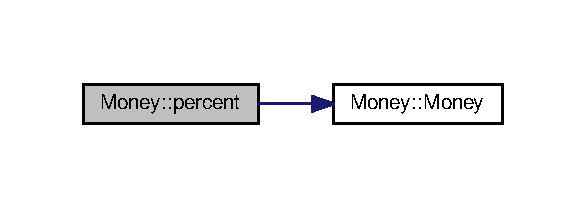
\includegraphics[width=281pt]{classMoney_ac8a69a07c01ce78261155d8262c4d132_cgraph}
\end{center}
\end{figure}




\subsection{Friends And Related Function Documentation}
\index{Money@{Money}!operator+@{operator+}}
\index{operator+@{operator+}!Money@{Money}}
\subsubsection[{\texorpdfstring{operator+}{operator+}}]{\setlength{\rightskip}{0pt plus 5cm}{\bf Money} operator+ (
\begin{DoxyParamCaption}
\item[{const {\bf Money} \&}]{amount1, }
\item[{const {\bf Money} \&}]{amount2}
\end{DoxyParamCaption}
)\hspace{0.3cm}{\ttfamily [friend]}}\hypertarget{classMoney_a050c2304648c379e54d793631adc3595}{}\label{classMoney_a050c2304648c379e54d793631adc3595}

\begin{DoxyCode}
206 \{
207    \hyperlink{classMoney}{Money} temp;
208    temp.\hyperlink{classMoney_a499d11509460668b7c262d9a58f7f310}{all\_cents} = amount1.\hyperlink{classMoney_a499d11509460668b7c262d9a58f7f310}{all\_cents} + amount2.\hyperlink{classMoney_a499d11509460668b7c262d9a58f7f310}{all\_cents};
209    \textcolor{keywordflow}{return} temp;
210 \}
\end{DoxyCode}
\index{Money@{Money}!operator-\/@{operator-\/}}
\index{operator-\/@{operator-\/}!Money@{Money}}
\subsubsection[{\texorpdfstring{operator-\/}{operator-}}]{\setlength{\rightskip}{0pt plus 5cm}{\bf Money} operator-\/ (
\begin{DoxyParamCaption}
\item[{const {\bf Money} \&}]{amount1, }
\item[{const {\bf Money} \&}]{amount2}
\end{DoxyParamCaption}
)\hspace{0.3cm}{\ttfamily [friend]}}\hypertarget{classMoney_afcc9c5cd27cc1c1b770681205a45cda0}{}\label{classMoney_afcc9c5cd27cc1c1b770681205a45cda0}

\begin{DoxyCode}
213 \{
214    \hyperlink{classMoney}{Money} temp;
215    temp.\hyperlink{classMoney_a499d11509460668b7c262d9a58f7f310}{all\_cents} = amount1.\hyperlink{classMoney_a499d11509460668b7c262d9a58f7f310}{all\_cents} - amount2.\hyperlink{classMoney_a499d11509460668b7c262d9a58f7f310}{all\_cents};
216    \textcolor{keywordflow}{return} temp;
217 \}
\end{DoxyCode}
\index{Money@{Money}!operator-\/@{operator-\/}}
\index{operator-\/@{operator-\/}!Money@{Money}}
\subsubsection[{\texorpdfstring{operator-\/}{operator-}}]{\setlength{\rightskip}{0pt plus 5cm}{\bf Money} operator-\/ (
\begin{DoxyParamCaption}
\item[{const {\bf Money} \&}]{amount}
\end{DoxyParamCaption}
)\hspace{0.3cm}{\ttfamily [friend]}}\hypertarget{classMoney_adeefac843a57c83f4ddd1125c5e001a0}{}\label{classMoney_adeefac843a57c83f4ddd1125c5e001a0}

\begin{DoxyCode}
220 \{
221    \hyperlink{classMoney}{Money} temp;
222    temp.\hyperlink{classMoney_a499d11509460668b7c262d9a58f7f310}{all\_cents} = -amount.\hyperlink{classMoney_a499d11509460668b7c262d9a58f7f310}{all\_cents};
223    \textcolor{keywordflow}{return} temp;
224 \}
\end{DoxyCode}
\index{Money@{Money}!operator$<$@{operator$<$}}
\index{operator$<$@{operator$<$}!Money@{Money}}
\subsubsection[{\texorpdfstring{operator$<$}{operator<}}]{\setlength{\rightskip}{0pt plus 5cm}bool operator$<$ (
\begin{DoxyParamCaption}
\item[{const {\bf Money} \&}]{amount1, }
\item[{const {\bf Money} \&}]{amount2}
\end{DoxyParamCaption}
)\hspace{0.3cm}{\ttfamily [friend]}}\hypertarget{classMoney_a31c79d588d6537e80efaa53e75747a61}{}\label{classMoney_a31c79d588d6537e80efaa53e75747a61}

\begin{DoxyCode}
232 \{
233    \textcolor{keywordflow}{return} (amount1.\hyperlink{classMoney_a499d11509460668b7c262d9a58f7f310}{all\_cents} < amount2.\hyperlink{classMoney_a499d11509460668b7c262d9a58f7f310}{all\_cents});
234 \}
\end{DoxyCode}
\index{Money@{Money}!operator$<$$<$@{operator$<$$<$}}
\index{operator$<$$<$@{operator$<$$<$}!Money@{Money}}
\subsubsection[{\texorpdfstring{operator$<$$<$}{operator<<}}]{\setlength{\rightskip}{0pt plus 5cm}ostream\& operator$<$$<$ (
\begin{DoxyParamCaption}
\item[{ostream \&}]{outs, }
\item[{const {\bf Money} \&}]{amount}
\end{DoxyParamCaption}
)\hspace{0.3cm}{\ttfamily [friend]}}\hypertarget{classMoney_a8ee9f1db0adb144c0d313ae202d06b3c}{}\label{classMoney_a8ee9f1db0adb144c0d313ae202d06b3c}

\begin{DoxyCode}
158 \{
159    \textcolor{keywordtype}{long} positive\_cents, dollars, cents;
160    positive\_cents = labs(amount.\hyperlink{classMoney_a499d11509460668b7c262d9a58f7f310}{all\_cents});
161    dollars = positive\_cents/100;
162    cents = positive\_cents%100;
163 
164    \textcolor{keywordflow}{if} (amount.\hyperlink{classMoney_a499d11509460668b7c262d9a58f7f310}{all\_cents} < 0)
165       outs << \textcolor{stringliteral}{"-$"} << dollars << \textcolor{charliteral}{'.'};
166    \textcolor{keywordflow}{else}
167       outs << \textcolor{stringliteral}{"$"} << dollars << \textcolor{charliteral}{'.'};
168 
169    \textcolor{keywordflow}{if} (cents < 10)
170       outs << \textcolor{charliteral}{'0'};
171    outs << cents;
172 
173    \textcolor{keywordflow}{return} outs;
174 \}
\end{DoxyCode}
\index{Money@{Money}!operator$<$=@{operator$<$=}}
\index{operator$<$=@{operator$<$=}!Money@{Money}}
\subsubsection[{\texorpdfstring{operator$<$=}{operator<=}}]{\setlength{\rightskip}{0pt plus 5cm}bool operator$<$= (
\begin{DoxyParamCaption}
\item[{const {\bf Money} \&}]{amount1, }
\item[{const {\bf Money} \&}]{amount2}
\end{DoxyParamCaption}
)\hspace{0.3cm}{\ttfamily [friend]}}\hypertarget{classMoney_ad45da707c7bee0cb12440a1c6ca3dc4b}{}\label{classMoney_ad45da707c7bee0cb12440a1c6ca3dc4b}

\begin{DoxyCode}
237 \{
238    \textcolor{keywordflow}{return} (amount1.\hyperlink{classMoney_a499d11509460668b7c262d9a58f7f310}{all\_cents} <= amount2.\hyperlink{classMoney_a499d11509460668b7c262d9a58f7f310}{all\_cents});
239 \}
\end{DoxyCode}
\index{Money@{Money}!operator==@{operator==}}
\index{operator==@{operator==}!Money@{Money}}
\subsubsection[{\texorpdfstring{operator==}{operator==}}]{\setlength{\rightskip}{0pt plus 5cm}bool operator== (
\begin{DoxyParamCaption}
\item[{const {\bf Money} \&}]{amount1, }
\item[{const {\bf Money} \&}]{amount2}
\end{DoxyParamCaption}
)\hspace{0.3cm}{\ttfamily [friend]}}\hypertarget{classMoney_adfbd10ed3dffab92c205b82c302357c6}{}\label{classMoney_adfbd10ed3dffab92c205b82c302357c6}

\begin{DoxyCode}
227 \{
228    \textcolor{keywordflow}{return} (amount1.\hyperlink{classMoney_a499d11509460668b7c262d9a58f7f310}{all\_cents} == amount2.\hyperlink{classMoney_a499d11509460668b7c262d9a58f7f310}{all\_cents});
229 \}
\end{DoxyCode}
\index{Money@{Money}!operator$>$@{operator$>$}}
\index{operator$>$@{operator$>$}!Money@{Money}}
\subsubsection[{\texorpdfstring{operator$>$}{operator>}}]{\setlength{\rightskip}{0pt plus 5cm}bool operator$>$ (
\begin{DoxyParamCaption}
\item[{const {\bf Money} \&}]{amount1, }
\item[{const {\bf Money} \&}]{amount2}
\end{DoxyParamCaption}
)\hspace{0.3cm}{\ttfamily [friend]}}\hypertarget{classMoney_adb213c2f9318ccaadd43a702ab25d614}{}\label{classMoney_adb213c2f9318ccaadd43a702ab25d614}

\begin{DoxyCode}
242 \{
243    \textcolor{keywordflow}{return} (amount1.\hyperlink{classMoney_a499d11509460668b7c262d9a58f7f310}{all\_cents} > amount2.\hyperlink{classMoney_a499d11509460668b7c262d9a58f7f310}{all\_cents});
244 \}
\end{DoxyCode}
\index{Money@{Money}!operator$>$=@{operator$>$=}}
\index{operator$>$=@{operator$>$=}!Money@{Money}}
\subsubsection[{\texorpdfstring{operator$>$=}{operator>=}}]{\setlength{\rightskip}{0pt plus 5cm}bool operator$>$= (
\begin{DoxyParamCaption}
\item[{const {\bf Money} \&}]{amount1, }
\item[{const {\bf Money} \&}]{amount2}
\end{DoxyParamCaption}
)\hspace{0.3cm}{\ttfamily [friend]}}\hypertarget{classMoney_af47b787881ddfdc6f98f3a86ba0a9d14}{}\label{classMoney_af47b787881ddfdc6f98f3a86ba0a9d14}

\begin{DoxyCode}
247 \{
248    \textcolor{keywordflow}{return} (amount1.\hyperlink{classMoney_a499d11509460668b7c262d9a58f7f310}{all\_cents} >= amount2.\hyperlink{classMoney_a499d11509460668b7c262d9a58f7f310}{all\_cents});
249 \}
\end{DoxyCode}
\index{Money@{Money}!operator$>$$>$@{operator$>$$>$}}
\index{operator$>$$>$@{operator$>$$>$}!Money@{Money}}
\subsubsection[{\texorpdfstring{operator$>$$>$}{operator>>}}]{\setlength{\rightskip}{0pt plus 5cm}istream\& operator$>$$>$ (
\begin{DoxyParamCaption}
\item[{istream \&}]{ins, }
\item[{{\bf Money} \&}]{amount}
\end{DoxyParamCaption}
)\hspace{0.3cm}{\ttfamily [friend]}}\hypertarget{classMoney_a4c8e628d575a860141c4fd4f2f38b186}{}\label{classMoney_a4c8e628d575a860141c4fd4f2f38b186}

\begin{DoxyCode}
115 \{
116    \textcolor{keywordtype}{char} one\_char, decimal\_point,
117       digit1, digit2; \textcolor{comment}{//digits for the amount of cents                                                     
                                                                                                       }
118    \textcolor{keywordtype}{long} dollars;
119    \textcolor{keywordtype}{int} cents;
120    \textcolor{keywordtype}{bool} negative;\textcolor{comment}{//set to true if input is negative.                                                       
                                                                                                       }
121 
122    ins >> one\_char;
123    \textcolor{keywordflow}{if} (one\_char == \textcolor{charliteral}{'-'})
124    \{
125       negative = \textcolor{keyword}{true};
126       ins >> one\_char; \textcolor{comment}{//read '$'                                                                          
                                                                                                       }
127    \}
128    \textcolor{keywordflow}{else}
129       negative = \textcolor{keyword}{false};
130    \textcolor{comment}{//if input is legal, then one\_char == '$'                                                               
                                                                                                       }
131 
132    ins >> dollars >> decimal\_point >> digit1 >> digit2;
133 
134    \textcolor{keywordflow}{if} ( one\_char != \textcolor{charliteral}{'$'} || decimal\_point != \textcolor{charliteral}{'.'}
135         || !isdigit(digit1) || !isdigit(digit2) )
136    \{
137       cout << \textcolor{stringliteral}{"Error illegal form for money input\(\backslash\)n"};
138       exit(1);
139    \}
140 
141    cents = \hyperlink{HW7_8cpp_a4a62e282ba4d4926583e5d206c744870}{digit\_to\_int}(digit1)*10 + \hyperlink{HW7_8cpp_a4a62e282ba4d4926583e5d206c744870}{digit\_to\_int}(digit2);
142 
143    amount.\hyperlink{classMoney_a499d11509460668b7c262d9a58f7f310}{all\_cents} = dollars*100 + cents;
144    \textcolor{keywordflow}{if} (negative)
145       amount.\hyperlink{classMoney_a499d11509460668b7c262d9a58f7f310}{all\_cents} = -amount.\hyperlink{classMoney_a499d11509460668b7c262d9a58f7f310}{all\_cents};
146 
147 
148    \textcolor{keywordflow}{return} ins;
149 \}
\end{DoxyCode}


\subsection{Member Data Documentation}
\index{Money@{Money}!all\+\_\+cents@{all\+\_\+cents}}
\index{all\+\_\+cents@{all\+\_\+cents}!Money@{Money}}
\subsubsection[{\texorpdfstring{all\+\_\+cents}{all_cents}}]{\setlength{\rightskip}{0pt plus 5cm}long Money\+::all\+\_\+cents\hspace{0.3cm}{\ttfamily [private]}}\hypertarget{classMoney_a499d11509460668b7c262d9a58f7f310}{}\label{classMoney_a499d11509460668b7c262d9a58f7f310}


The documentation for this class was generated from the following file\+:\begin{DoxyCompactItemize}
\item 
\hyperlink{HW7_8cpp}{H\+W7.\+cpp}\end{DoxyCompactItemize}

\chapter{File Documentation}
\hypertarget{HW7_8cpp}{}\section{H\+W7.\+cpp File Reference}
\label{HW7_8cpp}\index{H\+W7.\+cpp@{H\+W7.\+cpp}}
{\ttfamily \#include $<$iostream$>$}\\*
{\ttfamily \#include $<$fstream$>$}\\*
{\ttfamily \#include $<$cstdlib$>$}\\*
{\ttfamily \#include $<$cctype$>$}\\*
Include dependency graph for H\+W7.\+cpp\+:
\nopagebreak
\begin{figure}[H]
\begin{center}
\leavevmode
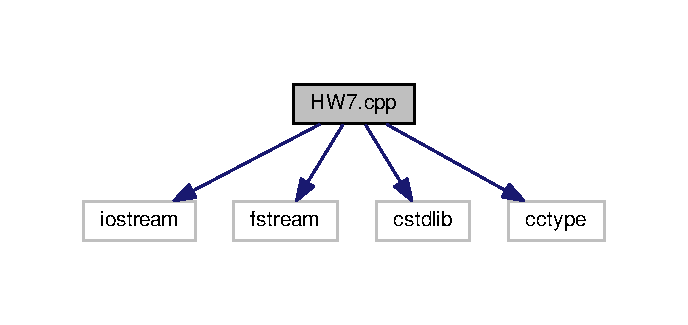
\includegraphics[width=330pt]{HW7_8cpp__incl}
\end{center}
\end{figure}
\subsection*{Classes}
\begin{DoxyCompactItemize}
\item 
class \hyperlink{classMoney}{Money}
\end{DoxyCompactItemize}
\subsection*{Functions}
\begin{DoxyCompactItemize}
\item 
int \hyperlink{HW7_8cpp_a4a62e282ba4d4926583e5d206c744870}{digit\+\_\+to\+\_\+int} (char c)
\item 
int \hyperlink{HW7_8cpp_ae66f6b31b5ad750f1fe042a706a4e3d4}{main} ()
\item 
istream \& \hyperlink{HW7_8cpp_a4c8e628d575a860141c4fd4f2f38b186}{operator$>$$>$} (istream \&ins, \hyperlink{classMoney}{Money} \&amount)
\item 
ostream \& \hyperlink{HW7_8cpp_a8ee9f1db0adb144c0d313ae202d06b3c}{operator$<$$<$} (ostream \&outs, const \hyperlink{classMoney}{Money} \&amount)
\item 
\hyperlink{classMoney}{Money} \hyperlink{HW7_8cpp_a050c2304648c379e54d793631adc3595}{operator+} (const \hyperlink{classMoney}{Money} \&amount1, const \hyperlink{classMoney}{Money} \&amount2)
\item 
\hyperlink{classMoney}{Money} \hyperlink{HW7_8cpp_afcc9c5cd27cc1c1b770681205a45cda0}{operator-\/} (const \hyperlink{classMoney}{Money} \&amount1, const \hyperlink{classMoney}{Money} \&amount2)
\item 
\hyperlink{classMoney}{Money} \hyperlink{HW7_8cpp_adeefac843a57c83f4ddd1125c5e001a0}{operator-\/} (const \hyperlink{classMoney}{Money} \&amount)
\item 
bool \hyperlink{HW7_8cpp_adfbd10ed3dffab92c205b82c302357c6}{operator==} (const \hyperlink{classMoney}{Money} \&amount1, const \hyperlink{classMoney}{Money} \&amount2)
\item 
bool \hyperlink{HW7_8cpp_a31c79d588d6537e80efaa53e75747a61}{operator$<$} (const \hyperlink{classMoney}{Money} \&amount1, const \hyperlink{classMoney}{Money} \&amount2)
\item 
bool \hyperlink{HW7_8cpp_ad45da707c7bee0cb12440a1c6ca3dc4b}{operator$<$=} (const \hyperlink{classMoney}{Money} \&amount1, const \hyperlink{classMoney}{Money} \&amount2)
\item 
bool \hyperlink{HW7_8cpp_adb213c2f9318ccaadd43a702ab25d614}{operator$>$} (const \hyperlink{classMoney}{Money} \&amount1, const \hyperlink{classMoney}{Money} \&amount2)
\item 
bool \hyperlink{HW7_8cpp_af47b787881ddfdc6f98f3a86ba0a9d14}{operator$>$=} (const \hyperlink{classMoney}{Money} \&amount1, const \hyperlink{classMoney}{Money} \&amount2)
\end{DoxyCompactItemize}


\subsection{Function Documentation}
\index{H\+W7.\+cpp@{H\+W7.\+cpp}!digit\+\_\+to\+\_\+int@{digit\+\_\+to\+\_\+int}}
\index{digit\+\_\+to\+\_\+int@{digit\+\_\+to\+\_\+int}!H\+W7.\+cpp@{H\+W7.\+cpp}}
\subsubsection[{\texorpdfstring{digit\+\_\+to\+\_\+int(char c)}{digit_to_int(char c)}}]{\setlength{\rightskip}{0pt plus 5cm}int digit\+\_\+to\+\_\+int (
\begin{DoxyParamCaption}
\item[{char}]{c}
\end{DoxyParamCaption}
)}\hypertarget{HW7_8cpp_a4a62e282ba4d4926583e5d206c744870}{}\label{HW7_8cpp_a4a62e282ba4d4926583e5d206c744870}

\begin{DoxyCode}
152 \{
153    \textcolor{keywordflow}{return} ( static\_cast<int>(c) - static\_cast<int>(\textcolor{charliteral}{'0'}) );
154 \}
\end{DoxyCode}
\index{H\+W7.\+cpp@{H\+W7.\+cpp}!main@{main}}
\index{main@{main}!H\+W7.\+cpp@{H\+W7.\+cpp}}
\subsubsection[{\texorpdfstring{main()}{main()}}]{\setlength{\rightskip}{0pt plus 5cm}int main (
\begin{DoxyParamCaption}
{}
\end{DoxyParamCaption}
)}\hypertarget{HW7_8cpp_ae66f6b31b5ad750f1fe042a706a4e3d4}{}\label{HW7_8cpp_ae66f6b31b5ad750f1fe042a706a4e3d4}

\begin{DoxyCode}
50 \{
51 \textcolor{comment}{/* Money amount;                                                                                           
                                                                                                       }
52 \textcolor{comment}{   ifstream in\_stream;                                                                                     
                                                                                                       }
53 \textcolor{comment}{   ofstream out\_stream;                                                                                    
                                                                                                       }
54 \textcolor{comment}{                                                                                                           
                                                                                                       }
55 \textcolor{comment}{   in\_stream.open("infile.dat");                                                                           
                                                                                                       }
56 \textcolor{comment}{   if (in\_stream.fail( ))                                                                                  
                                                                                                       }
57 \textcolor{comment}{   \{                                                                                                       
                                                                                                       }
58 \textcolor{comment}{      cout << "Input file opening failed.\(\backslash\)n";                                                              
                                                                                                       }
59 \textcolor{comment}{      exit(1);}
60 \textcolor{comment}{   \}                                                                                                       
                                                                                                       }
61 \textcolor{comment}{                                                                                                           
                                                                                                       }
62 \textcolor{comment}{   out\_stream.open("outfile.dat");                                                                         
                                                                                                       }
63 \textcolor{comment}{   if (out\_stream.fail( ))                                                                                 
                                                                                                       }
64 \textcolor{comment}{   \{                                                                                                       
                                                                                                       }
65 \textcolor{comment}{      cout << "Output file opening failed.\(\backslash\)n";                                                             
                                                                                                       }
66 \textcolor{comment}{      exit(1);                                                                                             
                                                                                                       }
67 \textcolor{comment}{   \}                                                                                                       
                                                                                                       }
68 \textcolor{comment}{                                                                                                           
                                                                                                       }
69 \textcolor{comment}{   in\_stream >> amount;                                                                                    
                                                                                                       }
70 \textcolor{comment}{   out\_stream << amount                                                                                    
                                                                                                       }
71 \textcolor{comment}{              << " copied from the file infile.dat.\(\backslash\)n";                                                    
                                                                                                       }
72 \textcolor{comment}{   cout << amount                                                                                          
                                                                                                       }
73 \textcolor{comment}{        << " copied from the file infile.dat.\(\backslash\)n";                                                          
                                                                                                       }
74 \textcolor{comment}{                                                                                                           
                                                                                                       }
75 \textcolor{comment}{   in\_stream.close( );                                                                                     
                                                                                                       }
76 \textcolor{comment}{   out\_stream.close( );                                                                                    
                                                                                                       }
77 \textcolor{comment}{*/}
78    \hyperlink{classMoney}{Money} m1(987, 45), m2(12);
79    cout << \textcolor{stringliteral}{"m1 = $"} << m1.get\_value() << endl;
80    cout << \textcolor{stringliteral}{"m2 = $"} << m2.get\_value() << endl;
81    \hyperlink{classMoney}{Money} m3(m1.percent(5));
82    \hyperlink{classMoney}{Money} m4(m2.percent(35));
83    cout << \textcolor{stringliteral}{"5% of m1 = $"} << m3.\hyperlink{classMoney_acee1d7ddca28c78740229a57cda5874f}{get\_value}() << endl;
84    cout << \textcolor{stringliteral}{"35% of m2 = $"} << m4.get\_value() << endl;
85    \textcolor{keywordflow}{if} (m3 == m4)
86       cout << \textcolor{stringliteral}{"They are equal!\(\backslash\)n"};
87    \textcolor{keywordflow}{else}
88       cout << \textcolor{stringliteral}{"They are NOT equal.\(\backslash\)n"};
89    \textcolor{keywordflow}{if} (m3 < m4)
90      cout << \textcolor{stringliteral}{"m3 is less than m4.\(\backslash\)n"};
91    \textcolor{keywordflow}{else}
92       cout << \textcolor{stringliteral}{"m4 is less than m3.\(\backslash\)n"};
93    \textcolor{keywordflow}{if} (m3 > m4)
94       cout << \textcolor{stringliteral}{"m3 is greater than m4.\(\backslash\)n"};
95    \textcolor{keywordflow}{else}
96       cout << \textcolor{stringliteral}{"m4 is greater than m3.\(\backslash\)n"};
97    \textcolor{keywordflow}{if} (m3 <= m4)
98       cout << \textcolor{stringliteral}{"m3 is less than or equal to m4.\(\backslash\)n"};
99    \textcolor{keywordflow}{else}
100       cout << \textcolor{stringliteral}{"m4 is less than or equal to m3.\(\backslash\)n"};
101    \textcolor{keywordflow}{if} (m3 >= m4)
102       cout << \textcolor{stringliteral}{"m3 is greater than or equal to m4.\(\backslash\)n"};
103    \textcolor{keywordflow}{else}
104       cout << \textcolor{stringliteral}{"m4 is greater than or equal to m3.\(\backslash\)n"};
105    \hyperlink{classMoney}{Money} m5(m1 - m2);
106    cout << \textcolor{stringliteral}{"m1 - m2 = $"} << m5.get\_value() << endl;
107    \hyperlink{classMoney}{Money} m6(m1 + m2);
108    cout << \textcolor{stringliteral}{"m1 + m2 = $"} << m6.get\_value() << endl;
109    \hyperlink{classMoney}{Money} m7(-m1);
110    cout << \textcolor{stringliteral}{"negative m1 = $"} << m7.get\_value() << endl;
111    \textcolor{keywordflow}{return} 0;
112 \}
\end{DoxyCode}


Here is the call graph for this function\+:
\nopagebreak
\begin{figure}[H]
\begin{center}
\leavevmode
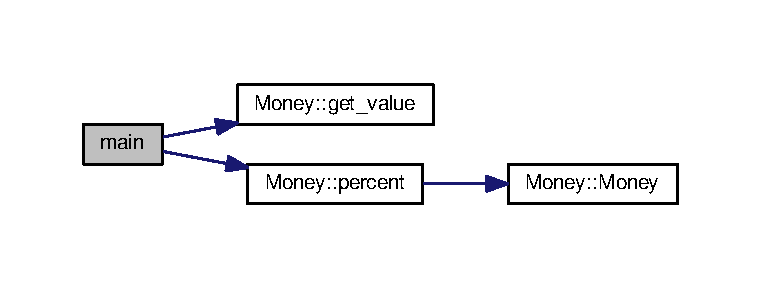
\includegraphics[width=350pt]{HW7_8cpp_ae66f6b31b5ad750f1fe042a706a4e3d4_cgraph}
\end{center}
\end{figure}


\index{H\+W7.\+cpp@{H\+W7.\+cpp}!operator+@{operator+}}
\index{operator+@{operator+}!H\+W7.\+cpp@{H\+W7.\+cpp}}
\subsubsection[{\texorpdfstring{operator+(const Money \&amount1, const Money \&amount2)}{operator+(const Money &amount1, const Money &amount2)}}]{\setlength{\rightskip}{0pt plus 5cm}{\bf Money} operator+ (
\begin{DoxyParamCaption}
\item[{const {\bf Money} \&}]{amount1, }
\item[{const {\bf Money} \&}]{amount2}
\end{DoxyParamCaption}
)}\hypertarget{HW7_8cpp_a050c2304648c379e54d793631adc3595}{}\label{HW7_8cpp_a050c2304648c379e54d793631adc3595}

\begin{DoxyCode}
206 \{
207    \hyperlink{classMoney}{Money} temp;
208    temp.\hyperlink{classMoney_a499d11509460668b7c262d9a58f7f310}{all\_cents} = amount1.\hyperlink{classMoney_a499d11509460668b7c262d9a58f7f310}{all\_cents} + amount2.\hyperlink{classMoney_a499d11509460668b7c262d9a58f7f310}{all\_cents};
209    \textcolor{keywordflow}{return} temp;
210 \}
\end{DoxyCode}
\index{H\+W7.\+cpp@{H\+W7.\+cpp}!operator-\/@{operator-\/}}
\index{operator-\/@{operator-\/}!H\+W7.\+cpp@{H\+W7.\+cpp}}
\subsubsection[{\texorpdfstring{operator-\/(const Money \&amount1, const Money \&amount2)}{operator-(const Money &amount1, const Money &amount2)}}]{\setlength{\rightskip}{0pt plus 5cm}{\bf Money} operator-\/ (
\begin{DoxyParamCaption}
\item[{const {\bf Money} \&}]{amount1, }
\item[{const {\bf Money} \&}]{amount2}
\end{DoxyParamCaption}
)}\hypertarget{HW7_8cpp_afcc9c5cd27cc1c1b770681205a45cda0}{}\label{HW7_8cpp_afcc9c5cd27cc1c1b770681205a45cda0}

\begin{DoxyCode}
213 \{
214    \hyperlink{classMoney}{Money} temp;
215    temp.\hyperlink{classMoney_a499d11509460668b7c262d9a58f7f310}{all\_cents} = amount1.\hyperlink{classMoney_a499d11509460668b7c262d9a58f7f310}{all\_cents} - amount2.\hyperlink{classMoney_a499d11509460668b7c262d9a58f7f310}{all\_cents};
216    \textcolor{keywordflow}{return} temp;
217 \}
\end{DoxyCode}
\index{H\+W7.\+cpp@{H\+W7.\+cpp}!operator-\/@{operator-\/}}
\index{operator-\/@{operator-\/}!H\+W7.\+cpp@{H\+W7.\+cpp}}
\subsubsection[{\texorpdfstring{operator-\/(const Money \&amount)}{operator-(const Money &amount)}}]{\setlength{\rightskip}{0pt plus 5cm}{\bf Money} operator-\/ (
\begin{DoxyParamCaption}
\item[{const {\bf Money} \&}]{amount}
\end{DoxyParamCaption}
)}\hypertarget{HW7_8cpp_adeefac843a57c83f4ddd1125c5e001a0}{}\label{HW7_8cpp_adeefac843a57c83f4ddd1125c5e001a0}

\begin{DoxyCode}
220 \{
221    \hyperlink{classMoney}{Money} temp;
222    temp.\hyperlink{classMoney_a499d11509460668b7c262d9a58f7f310}{all\_cents} = -amount.\hyperlink{classMoney_a499d11509460668b7c262d9a58f7f310}{all\_cents};
223    \textcolor{keywordflow}{return} temp;
224 \}
\end{DoxyCode}
\index{H\+W7.\+cpp@{H\+W7.\+cpp}!operator$<$@{operator$<$}}
\index{operator$<$@{operator$<$}!H\+W7.\+cpp@{H\+W7.\+cpp}}
\subsubsection[{\texorpdfstring{operator$<$(const Money \&amount1, const Money \&amount2)}{operator<(const Money &amount1, const Money &amount2)}}]{\setlength{\rightskip}{0pt plus 5cm}bool operator$<$ (
\begin{DoxyParamCaption}
\item[{const {\bf Money} \&}]{amount1, }
\item[{const {\bf Money} \&}]{amount2}
\end{DoxyParamCaption}
)}\hypertarget{HW7_8cpp_a31c79d588d6537e80efaa53e75747a61}{}\label{HW7_8cpp_a31c79d588d6537e80efaa53e75747a61}

\begin{DoxyCode}
232 \{
233    \textcolor{keywordflow}{return} (amount1.\hyperlink{classMoney_a499d11509460668b7c262d9a58f7f310}{all\_cents} < amount2.\hyperlink{classMoney_a499d11509460668b7c262d9a58f7f310}{all\_cents});
234 \}
\end{DoxyCode}
\index{H\+W7.\+cpp@{H\+W7.\+cpp}!operator$<$$<$@{operator$<$$<$}}
\index{operator$<$$<$@{operator$<$$<$}!H\+W7.\+cpp@{H\+W7.\+cpp}}
\subsubsection[{\texorpdfstring{operator$<$$<$(ostream \&outs, const Money \&amount)}{operator<<(ostream &outs, const Money &amount)}}]{\setlength{\rightskip}{0pt plus 5cm}ostream\& operator$<$$<$ (
\begin{DoxyParamCaption}
\item[{ostream \&}]{outs, }
\item[{const {\bf Money} \&}]{amount}
\end{DoxyParamCaption}
)}\hypertarget{HW7_8cpp_a8ee9f1db0adb144c0d313ae202d06b3c}{}\label{HW7_8cpp_a8ee9f1db0adb144c0d313ae202d06b3c}

\begin{DoxyCode}
158 \{
159    \textcolor{keywordtype}{long} positive\_cents, dollars, cents;
160    positive\_cents = labs(amount.\hyperlink{classMoney_a499d11509460668b7c262d9a58f7f310}{all\_cents});
161    dollars = positive\_cents/100;
162    cents = positive\_cents%100;
163 
164    \textcolor{keywordflow}{if} (amount.\hyperlink{classMoney_a499d11509460668b7c262d9a58f7f310}{all\_cents} < 0)
165       outs << \textcolor{stringliteral}{"-$"} << dollars << \textcolor{charliteral}{'.'};
166    \textcolor{keywordflow}{else}
167       outs << \textcolor{stringliteral}{"$"} << dollars << \textcolor{charliteral}{'.'};
168 
169    \textcolor{keywordflow}{if} (cents < 10)
170       outs << \textcolor{charliteral}{'0'};
171    outs << cents;
172 
173    \textcolor{keywordflow}{return} outs;
174 \}
\end{DoxyCode}
\index{H\+W7.\+cpp@{H\+W7.\+cpp}!operator$<$=@{operator$<$=}}
\index{operator$<$=@{operator$<$=}!H\+W7.\+cpp@{H\+W7.\+cpp}}
\subsubsection[{\texorpdfstring{operator$<$=(const Money \&amount1, const Money \&amount2)}{operator<=(const Money &amount1, const Money &amount2)}}]{\setlength{\rightskip}{0pt plus 5cm}bool operator$<$= (
\begin{DoxyParamCaption}
\item[{const {\bf Money} \&}]{amount1, }
\item[{const {\bf Money} \&}]{amount2}
\end{DoxyParamCaption}
)}\hypertarget{HW7_8cpp_ad45da707c7bee0cb12440a1c6ca3dc4b}{}\label{HW7_8cpp_ad45da707c7bee0cb12440a1c6ca3dc4b}

\begin{DoxyCode}
237 \{
238    \textcolor{keywordflow}{return} (amount1.\hyperlink{classMoney_a499d11509460668b7c262d9a58f7f310}{all\_cents} <= amount2.\hyperlink{classMoney_a499d11509460668b7c262d9a58f7f310}{all\_cents});
239 \}
\end{DoxyCode}
\index{H\+W7.\+cpp@{H\+W7.\+cpp}!operator==@{operator==}}
\index{operator==@{operator==}!H\+W7.\+cpp@{H\+W7.\+cpp}}
\subsubsection[{\texorpdfstring{operator==(const Money \&amount1, const Money \&amount2)}{operator==(const Money &amount1, const Money &amount2)}}]{\setlength{\rightskip}{0pt plus 5cm}bool operator== (
\begin{DoxyParamCaption}
\item[{const {\bf Money} \&}]{amount1, }
\item[{const {\bf Money} \&}]{amount2}
\end{DoxyParamCaption}
)}\hypertarget{HW7_8cpp_adfbd10ed3dffab92c205b82c302357c6}{}\label{HW7_8cpp_adfbd10ed3dffab92c205b82c302357c6}

\begin{DoxyCode}
227 \{
228    \textcolor{keywordflow}{return} (amount1.\hyperlink{classMoney_a499d11509460668b7c262d9a58f7f310}{all\_cents} == amount2.\hyperlink{classMoney_a499d11509460668b7c262d9a58f7f310}{all\_cents});
229 \}
\end{DoxyCode}
\index{H\+W7.\+cpp@{H\+W7.\+cpp}!operator$>$@{operator$>$}}
\index{operator$>$@{operator$>$}!H\+W7.\+cpp@{H\+W7.\+cpp}}
\subsubsection[{\texorpdfstring{operator$>$(const Money \&amount1, const Money \&amount2)}{operator>(const Money &amount1, const Money &amount2)}}]{\setlength{\rightskip}{0pt plus 5cm}bool operator$>$ (
\begin{DoxyParamCaption}
\item[{const {\bf Money} \&}]{amount1, }
\item[{const {\bf Money} \&}]{amount2}
\end{DoxyParamCaption}
)}\hypertarget{HW7_8cpp_adb213c2f9318ccaadd43a702ab25d614}{}\label{HW7_8cpp_adb213c2f9318ccaadd43a702ab25d614}

\begin{DoxyCode}
242 \{
243    \textcolor{keywordflow}{return} (amount1.\hyperlink{classMoney_a499d11509460668b7c262d9a58f7f310}{all\_cents} > amount2.\hyperlink{classMoney_a499d11509460668b7c262d9a58f7f310}{all\_cents});
244 \}
\end{DoxyCode}
\index{H\+W7.\+cpp@{H\+W7.\+cpp}!operator$>$=@{operator$>$=}}
\index{operator$>$=@{operator$>$=}!H\+W7.\+cpp@{H\+W7.\+cpp}}
\subsubsection[{\texorpdfstring{operator$>$=(const Money \&amount1, const Money \&amount2)}{operator>=(const Money &amount1, const Money &amount2)}}]{\setlength{\rightskip}{0pt plus 5cm}bool operator$>$= (
\begin{DoxyParamCaption}
\item[{const {\bf Money} \&}]{amount1, }
\item[{const {\bf Money} \&}]{amount2}
\end{DoxyParamCaption}
)}\hypertarget{HW7_8cpp_af47b787881ddfdc6f98f3a86ba0a9d14}{}\label{HW7_8cpp_af47b787881ddfdc6f98f3a86ba0a9d14}

\begin{DoxyCode}
247 \{
248    \textcolor{keywordflow}{return} (amount1.\hyperlink{classMoney_a499d11509460668b7c262d9a58f7f310}{all\_cents} >= amount2.\hyperlink{classMoney_a499d11509460668b7c262d9a58f7f310}{all\_cents});
249 \}
\end{DoxyCode}
\index{H\+W7.\+cpp@{H\+W7.\+cpp}!operator$>$$>$@{operator$>$$>$}}
\index{operator$>$$>$@{operator$>$$>$}!H\+W7.\+cpp@{H\+W7.\+cpp}}
\subsubsection[{\texorpdfstring{operator$>$$>$(istream \&ins, Money \&amount)}{operator>>(istream &ins, Money &amount)}}]{\setlength{\rightskip}{0pt plus 5cm}istream\& operator$>$$>$ (
\begin{DoxyParamCaption}
\item[{istream \&}]{ins, }
\item[{{\bf Money} \&}]{amount}
\end{DoxyParamCaption}
)}\hypertarget{HW7_8cpp_a4c8e628d575a860141c4fd4f2f38b186}{}\label{HW7_8cpp_a4c8e628d575a860141c4fd4f2f38b186}

\begin{DoxyCode}
115 \{
116    \textcolor{keywordtype}{char} one\_char, decimal\_point,
117       digit1, digit2; \textcolor{comment}{//digits for the amount of cents                                                     
                                                                                                       }
118    \textcolor{keywordtype}{long} dollars;
119    \textcolor{keywordtype}{int} cents;
120    \textcolor{keywordtype}{bool} negative;\textcolor{comment}{//set to true if input is negative.                                                       
                                                                                                       }
121 
122    ins >> one\_char;
123    \textcolor{keywordflow}{if} (one\_char == \textcolor{charliteral}{'-'})
124    \{
125       negative = \textcolor{keyword}{true};
126       ins >> one\_char; \textcolor{comment}{//read '$'                                                                          
                                                                                                       }
127    \}
128    \textcolor{keywordflow}{else}
129       negative = \textcolor{keyword}{false};
130    \textcolor{comment}{//if input is legal, then one\_char == '$'                                                               
                                                                                                       }
131 
132    ins >> dollars >> decimal\_point >> digit1 >> digit2;
133 
134    \textcolor{keywordflow}{if} ( one\_char != \textcolor{charliteral}{'$'} || decimal\_point != \textcolor{charliteral}{'.'}
135         || !isdigit(digit1) || !isdigit(digit2) )
136    \{
137       cout << \textcolor{stringliteral}{"Error illegal form for money input\(\backslash\)n"};
138       exit(1);
139    \}
140 
141    cents = \hyperlink{HW7_8cpp_a4a62e282ba4d4926583e5d206c744870}{digit\_to\_int}(digit1)*10 + \hyperlink{HW7_8cpp_a4a62e282ba4d4926583e5d206c744870}{digit\_to\_int}(digit2);
142 
143    amount.\hyperlink{classMoney_a499d11509460668b7c262d9a58f7f310}{all\_cents} = dollars*100 + cents;
144    \textcolor{keywordflow}{if} (negative)
145       amount.\hyperlink{classMoney_a499d11509460668b7c262d9a58f7f310}{all\_cents} = -amount.\hyperlink{classMoney_a499d11509460668b7c262d9a58f7f310}{all\_cents};
146 
147 
148    \textcolor{keywordflow}{return} ins;
149 \}
\end{DoxyCode}


Here is the call graph for this function\+:
\nopagebreak
\begin{figure}[H]
\begin{center}
\leavevmode
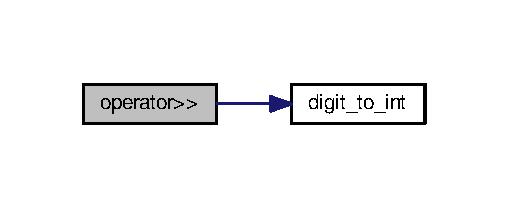
\includegraphics[width=244pt]{HW7_8cpp_a4c8e628d575a860141c4fd4f2f38b186_cgraph}
\end{center}
\end{figure}



%--- End generated contents ---

% Index
\backmatter
\newpage
\phantomsection
\clearemptydoublepage
\addcontentsline{toc}{chapter}{Index}
\printindex

\end{document}
